% !TeX spellcheck = en_GB

\section{CLI Tool}
Write much of this stuff in the appendix.

\subsection{Scoring Model}

Only valid ResultSamples are given a score. Parameters to be scored:
\begin{itemize}
	\item RightCellCombinationsForcedCount
	\item maxSumOfVarsInPyramidCount 	
	\item maxNumberOfVarsPerCellCount
	\item maxSumOfProductionsCount
\end{itemize}

\noindent Maybe add a diversity criterion = homogeneity of the cells to the scoring matrix.

\begin{table}[H]
	\centering
	\begin{tabular}{|l|c|c|c|c|c|l|}
		\hline
		\multicolumn{1}{|c|}{\multirow{2}{*}{Parameter}} & \multicolumn{6}{c|}{Points}                                                          \\ \cline{2-7} 
		\multicolumn{1}{|c|}{}                           & 2          & 4           & 6           & 8           & 10          & -100            \\ \hline
		cellCombinationsForced                           & {[}0,10{]} & {[}11,20{]} & {[}21,30{]} & {[}41,50{]} & {[}31,40{]} & \textgreater 50 \\ \hline
		sumVarsInPyramid                                 & {[}0,10{]} & {[}11,20{]} & {[}21,30{]} & {[}41,50{]} & {[}31,40{]} & \textgreater 50 \\ \hline
		maxVarsPerCell                                   & {[}5,5{]}  & {[}4,4{]}   & {[}1,1{]}   & {[}3,3{]}   & {[}2,2{]}   & \textgreater 5  \\ \hline
		sumProductions                                   & {[}1,2{]}  & {[}3,4{]}   & {[}5,6{]}   & {[}9,10{]}  & {[}7,8{]}   & \textgreater 10 \\ \hline
	\end{tabular}
	\caption{Scoring of the different parameter values}
	\label{scoring}
\end{table}



\noindent Based on table \ref{scoring} each result sample is scored. Out of the \#??? best result samples one can choose.\\
The result will be normalized to the maximum possible points -> range 0.0 to 1.0. 


\subsection{Short Requirements Specification}

\noindent Generating the latex code and storing it in .tex-file. Then converting the .tex-file to .pdf-file via:\\
Runtime rt = Runtime.getRuntime();\\
Process pr = rt.exec("pdflatex mydoc.tex");\\
Process pr = rt.exec("pdflatex mydoc.tex");\\
Process pr = rt.exec("pdflatex mydoc.tex");\\
The triple invocation of LaTeX is to ensure that all references have been properly resolved and any page layout changes due to inserting the references have been accounted for. [http://www.arakhne.org/autolatex/]

\pagebreak
\subsubsection{Exam Exercises}
4-tuples $exercise = (grammar,\ word,\ parse\ table,\ derivation\ tree)$ that needs to be printed.
\begin{center} 
	\begin{tabular}{l}$A\rightarrow BC~|~a~|~b~~$\\ 
		$B\rightarrow b~|~BB~~$\\ 
		$C\rightarrow c~|~AC~~$\\ 
		$S\rightarrow CB~|~AA~|~AC~~$\\ 
	\end{tabular} 
\end{center}
\begin{center}
	\resizebox{\linewidth}{!}{
		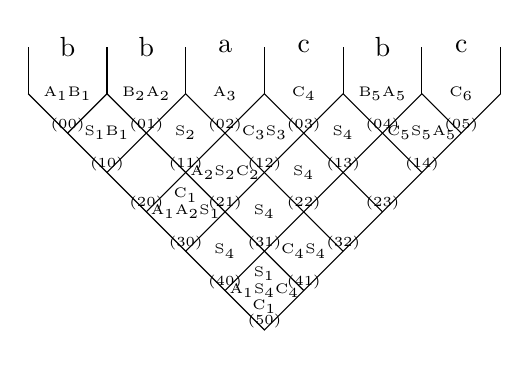
\begin{tikzpicture}[baseline]
		\newcommand{\myfontvars}[1]{
			\fontsize{4.9}{12}\selectfont{#1}
		}\newcommand{\myfontnumbering}[1]{
			\fontsize{2.5}{12}\selectfont{#1}
		}%Outer hull
		%Tip of the pyramid
		\coordinate (tip) at (3,-3);
		\foreach \i in {0,...,6} {
			\coordinate (\i) at (\i,0);
		}
		%Draw the left and right line of the pyramid pointing downwards
		\draw (0) -- (tip) -- (6);
		%Grid lines direction down-left to top-right
		\coordinate (dl1) at (0.5,-0.5);
		\coordinate (dl2) at (1.0,-1.0);
		\coordinate (dl3) at (1.5,-1.5);
		\coordinate (dl4) at (2.0,-2.0);
		\coordinate (dl5) at (2.5,-2.5);
		\draw (dl1) -- (1,0);
		\draw (dl2) -- (2,0);
		\draw (dl3) -- (3,0);
		\draw (dl4) -- (4,0);
		\draw (dl5) -- (5,0);
		%Grid lines direction down-right to top-left
		\coordinate (dr1) at (3.5,-2.5);
		\coordinate (dr2) at (4.0,-2.0);
		\coordinate (dr3) at (4.5,-1.5);
		\coordinate (dr4) at (5.0,-1.0);
		\coordinate (dr5) at (5.5,-0.5);
		\draw (dr1) -- (1,0);
		\draw (dr2) -- (2,0);
		\draw (dr3) -- (3,0);
		\draw (dr4) -- (4,0);
		\draw (dr5) -- (5,0);
		%Small lines at the top
		\coordinate (top0) at (0.0,0.0);
		\coordinate (top1) at (1.0,0.0);
		\coordinate (top2) at (2.0,0.0);
		\coordinate (top3) at (3.0,0.0);
		\coordinate (top4) at (4.0,0.0);
		\coordinate (top5) at (5.0,0.0);
		\coordinate (top6) at (6.0,0.0);
		\coordinate (topUpper0) at (0.0,0.6);
		\coordinate (topUpper1) at (1.0,0.6);
		\coordinate (topUpper2) at (2.0,0.6);
		\coordinate (topUpper3) at (3.0,0.6);
		\coordinate (topUpper4) at (4.0,0.6);
		\coordinate (topUpper5) at (5.0,0.6);
		\coordinate (topUpper6) at (6.0,0.6);
		\draw (top0) -- (topUpper0);
		\draw (top1) -- (topUpper1);
		\draw (top2) -- (topUpper2);
		\draw (top3) -- (topUpper3);
		\draw (top4) -- (topUpper4);
		\draw (top5) -- (topUpper5);
		\draw (top6) -- (topUpper6);
		%The string
		\coordinate (w0) at (0.5,0.6);
		\coordinate (w1) at (1.5,0.6);
		\coordinate (w2) at (2.5,0.6);
		\coordinate (w3) at (3.5,0.6);
		\coordinate (w4) at (4.5,0.6);
		\coordinate (w5) at (5.5,0.6);
		\node [] at (w0) {b};
		\node [] at (w1) {b};
		\node [] at (w2) {a};
		\node [] at (w3) {c};
		\node [] at (w4) {b};
		\node [] at (w5) {c};
		% Variables in the cells
		%cells00
		\coordinate (center00) at (0.5,0.0);
		\node [below=0.18cm] at (center00) {\myfontnumbering{$(00)$}};
		\node [] at (center00) {\myfontvars{A$_1$B$_1$}};
		%cells01
		\coordinate (center01) at (1.5,0.0);
		\node [below=0.18cm] at (center01) {\myfontnumbering{$(01)$}};
		\node [] at (center01) {\myfontvars{B$_2$A$_2$}};
		%cells02
		\coordinate (center02) at (2.5,0.0);
		\node [below=0.18cm] at (center02) {\myfontnumbering{$(02)$}};
		\node [] at (center02) {\myfontvars{A$_3$}};
		%cells03
		\coordinate (center03) at (3.5,0.0);
		\node [below=0.18cm] at (center03) {\myfontnumbering{$(03)$}};
		\node [] at (center03) {\myfontvars{C$_4$}};
		%cells04
		\coordinate (center04) at (4.5,0.0);
		\node [below=0.18cm] at (center04) {\myfontnumbering{$(04)$}};
		\node [] at (center04) {\myfontvars{B$_5$A$_5$}};
		%cells05
		\coordinate (center05) at (5.5,0.0);
		\node [below=0.18cm] at (center05) {\myfontnumbering{$(05)$}};
		\node [] at (center05) {\myfontvars{C$_6$}};
		%cells10
		\coordinate (center10) at (1.0,-0.5);
		\node [below=0.18cm] at (center10) {\myfontnumbering{$(10)$}};
		\node [] at (center10) {\myfontvars{S$_1$B$_1$}};
		%cells11
		\coordinate (center11) at (2.0,-0.5);
		\node [below=0.18cm] at (center11) {\myfontnumbering{$(11)$}};
		\node [] at (center11) {\myfontvars{S$_2$}};
		%cells12
		\coordinate (center12) at (3.0,-0.5);
		\node [below=0.18cm] at (center12) {\myfontnumbering{$(12)$}};
		\node [] at (center12) {\myfontvars{C$_3$S$_3$}};
		%cells13
		\coordinate (center13) at (4.0,-0.5);
		\node [below=0.18cm] at (center13) {\myfontnumbering{$(13)$}};
		\node [] at (center13) {\myfontvars{S$_4$}};
		%cells14
		\coordinate (center14) at (5.0,-0.5);
		\node [below=0.18cm] at (center14) {\myfontnumbering{$(14)$}};
		\node [] at (center14) {\myfontvars{C$_5$S$_5$A$_5$}};
		%cells20
		\coordinate (center20) at (1.5,-1.0);
		\node [below=0.18cm] at (center20) {\myfontnumbering{$(20)$}};
		%cells21
		\coordinate (center21) at (2.5,-1.0);
		\node [below=0.18cm] at (center21) {\myfontnumbering{$(21)$}};
		\node [] at (center21) {\myfontvars{A$_2$S$_2$C$_2$}};
		%cells22
		\coordinate (center22) at (3.5,-1.0);
		\node [below=0.18cm] at (center22) {\myfontnumbering{$(22)$}};
		\node [] at (center22) {\myfontvars{S$_4$}};
		%cells23
		\coordinate (center23) at (4.5,-1.0);
		\node [below=0.18cm] at (center23) {\myfontnumbering{$(23)$}};
		%cells30
		\coordinate (center30) at (2.0,-1.5);
		\node [below=0.18cm] at (center30) {\myfontnumbering{$(30)$}};
		\node [] at (center30) {\myfontvars{A$_1$A$_2$S$_1$}};
		\node [above] at (center30) {\myfontvars{C$_1$}};
		%cells31
		\coordinate (center31) at (3.0,-1.5);
		\node [below=0.18cm] at (center31) {\myfontnumbering{$(31)$}};
		\node [] at (center31) {\myfontvars{S$_4$}};
		%cells32
		\coordinate (center32) at (4.0,-1.5);
		\node [below=0.18cm] at (center32) {\myfontnumbering{$(32)$}};
		%cells40
		\coordinate (center40) at (2.5,-2.0);
		\node [below=0.18cm] at (center40) {\myfontnumbering{$(40)$}};
		\node [] at (center40) {\myfontvars{S$_4$}};
		%cells41
		\coordinate (center41) at (3.5,-2.0);
		\node [below=0.18cm] at (center41) {\myfontnumbering{$(41)$}};
		\node [] at (center41) {\myfontvars{C$_4$S$_4$}};
		%cells50
		\coordinate (center50) at (3.0,-2.5);
		\node [below=0.18cm] at (center50) {\myfontnumbering{$(50)$}};
		\node [] at (center50) {\myfontvars{A$_1$S$_4$C$_4$}};
		\node [above] at (center50) {\myfontvars{S$_1$}};
		\node [below] at (center50) {\myfontvars{C$_1$}};
		\end{tikzpicture}
	}
\end{center}
\pagebreak
Maybe don't add the $Tree$ here. It is only needed as one part of the output of an $exercise$.
\begin{center}
	\resizebox{.6\linewidth}{!}{
		\begin{tikzpicture}[-,>=stealth',shorten >=1pt,auto,node distance=2cm,
		semithick]%,initial text={}]
		\tikzstyle{every state}=[fill=white,draw=black,text=black]
		
		\node     (I)            {$S1$};
		\node				(I') [below left of=I] {};
		\node (B) [left of=I']  {$A1$};
		\node (B1) [below of=B] {$c$};
		\node (C) [below right  of=I]       {$B6$};
		\node (D) [below right of=C]  {$B7$};
		\node (D2) [below left of=C]  {$C4$};
		\node (E) [below right of=D]  {$B8$};
		\node (F1) [below of=E]  {$b$};
		\node (E1) [below of=D]  {$C7$};
		\node (E3) [below of=D2]  {$C5$};
		\node (E2) [below left of=D2]  {$A2$};
		\node (F) [below  of=E1]  {$c$};
		\node (F3) [below of=E3]  {$A5$};
		\node (G1) [below  of=F3]  {$a$};
		\node (F2) [below right of=E3]  {$C6$};
		\node (G2) [below  of=F2]  {$c$};
		\node (H1) [below of=E2]  {$A3$};
		\node (H2) [below left of=E2]  {$B2$};
		\node (H3) [below left of=H2]  {$b$};
		\node (J1) [below of=H1]  {$A4$};
		\node (K1) [below of=J1]  {$a$};
		\node (J2) [below left of=H1]  {$B3$};
		\node (K3) [below of=J2]  {$b$};
		
		\path 
		(I) edge   node {$ $}   (B)
		(I) edge   node {$ $}   (C)
		(B) edge   node {$ $}   (B1)
		(C) edge   node {$ $}   (D)
		(D) edge   node {$ $}   (E)
		(C) edge   node {$ $}   (D2)
		(D2) edge   node {$ $}   (E3)
		(D) edge   node {$ $}   (E1)
		(D2) edge   node {$ $}   (E2)
		(E1) edge   node {$ $}   (F)
		(E) edge   node {$ $}   (F1)
		(E3) edge   node {$ $}   (F3)
		(E3) edge   node {$ $}   (F2)
		(F2) edge   node {$ $}   (G2)
		(F3) edge   node {$ $}   (G1)
		(E2) edge   node {$ $}   (H2)
		(E2) edge   node {$ $}   (H1)
		(H2) edge   node {$ $}   (H3)
		(H1) edge   node {$ $}   (J2)
		(H1) edge   node {$ $}   (J1)
		(J1) edge   node {$ $}   (K1)
		(J2) edge   node {$ $}   (K3)
		;
		
		\end{tikzpicture}
	}
	
\end{center}



\pagebreak
\subsection{Overview - UML}

UML-Diagramm showing the general idea of the implementation.\\
List noteworthy used libraries here, too.\\
Maybe some information out of the statistics tool of IntelliJ.

\subsubsection{UML: More Detail 1}
\subsubsection{UML: More Detail 2}

\pagebreak
\subsection{User Interaction}

\noindent Here the specific must can do's are explained with short examples.
\subsubsection{Use Case 1}
\subsubsection{Use Case i}

\pagebreak